\documentclass{beamer}

\usepackage[frenchb]{babel}
\usepackage[T1]{fontenc}
\usepackage[utf8]{inputenc}

\usepackage{default}
\usepackage{pslatex}
\usepackage{graphicx}
\usepackage{tikz}
\usepackage{pgfplots}
% \usepackage{algorithmic}
\usepackage{multicol}

\usetheme{Warsaw}
\usetikzlibrary{arrows}
\pagestyle{empty}
\definecolor{qqwuqq}{rgb}{0,0.39,0}
\definecolor{xdxdff}{rgb}{0.49,0.49,1}
\definecolor{uququq}{rgb}{0.25,0.25,0.25}
\definecolor{qqqqff}{rgb}{0,0,1}
\setcounter{tocdepth}{4}

\title{Comment simuler numériquement la géomorphologie alpine ?}
\subtitle{Sujet de TPE}
\author{Gros Alexis, Manceau Thibaut, Porteries Tristan}
% \logo{
\includegraphics[height=0.5cm]{blender.png}}

\makeindex

\useoutertheme{infolines}

\begin{document}

% Titre
\frame{\titlepage}

% Sommaire
\begin{frame}{Sommaire}
  \begin{multicols}{2}
    \small \tableofcontents
  \end{multicols}
\end{frame}

\section{Les phénomènes géormophologiques}
\subsection{La subduction et l'obduction}
\begin{frame}
  \begin{figure}
    \begin{center}
      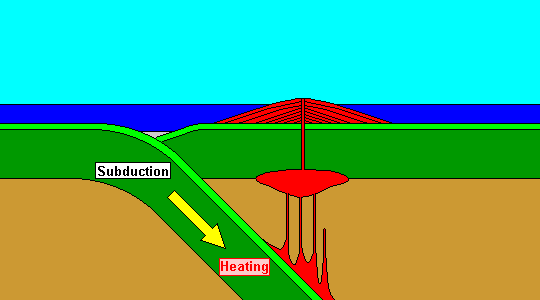
\includegraphics[width=6cm]{Images/subduction.png}
      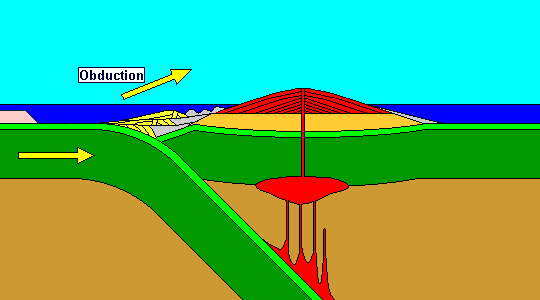
\includegraphics[width=6cm]{Images/obduction.png}
      \caption{A gauche le subduction et à droite l'obduction.}
    \end{center}
  \end{figure}
\end{frame}

\section{Les altérations}
\subsection{Les altérations physiques}
\begin{frame}
  \begin{center}
    \begin{figure}
      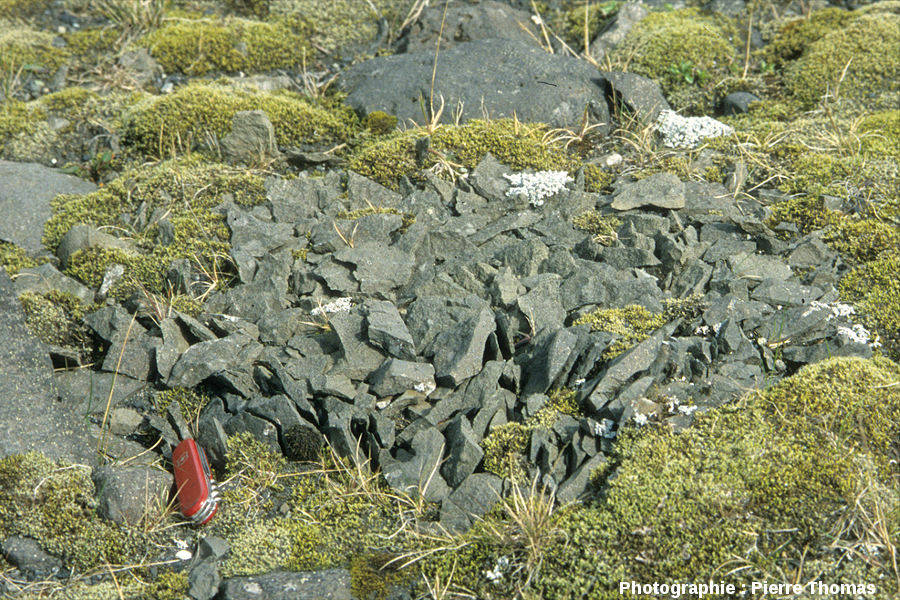
\includegraphics[width=4.5cm]{Images/Diapos/Alteration/Physique/cryoclastie.jpg}
      \caption{Cryoclastie}
    \end{figure}
  \end{center}
  \begin{center}
    \begin{figure}
      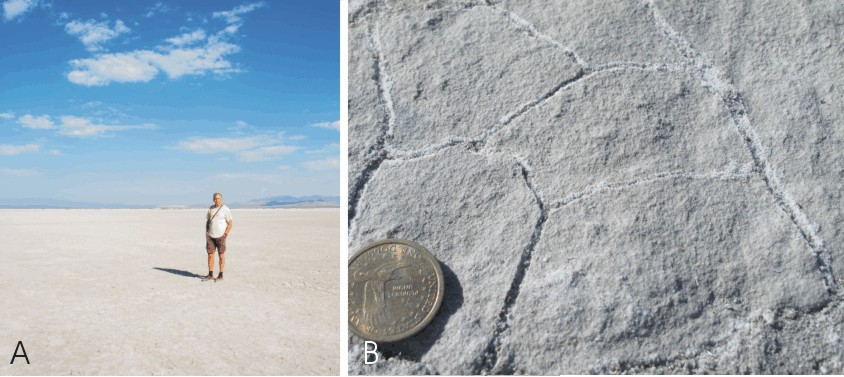
\includegraphics[width=7.4cm]{Images/Diapos/Alteration/Physique/haloclastie3.jpg}
      \caption{Haloclastie}
    \end{figure}
  \end{center}
\end{frame}

\subsection{Les altérations chimiques}
\begin{frame}
  \begin{center}
    \begin{figure}
      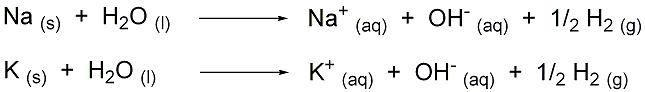
\includegraphics[width=7cm]{Images/Diapos/Alteration/Chimiques/hydrolyse.png}
      \caption{Hydratation de molécules de sodium et de potassium.}
    \end{figure}
  \end{center}
  \begin{center}
    \begin{figure}
      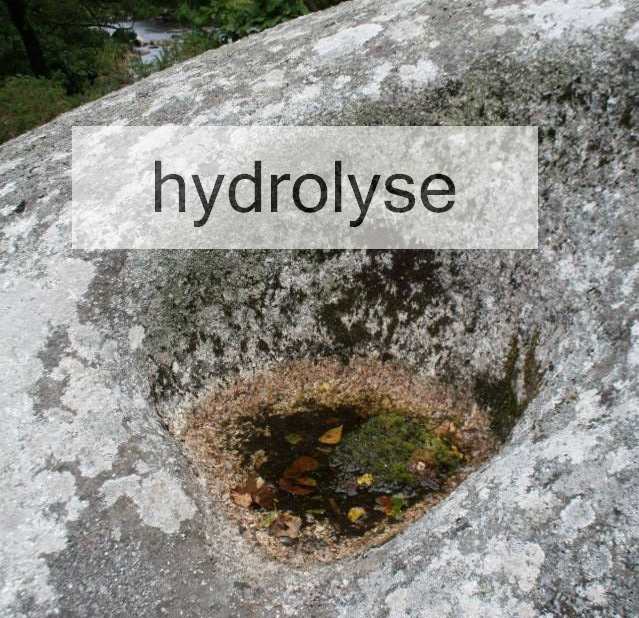
\includegraphics[width=5cm]{Images/Diapos/Alteration/Chimiques/hydrolyse.jpeg}
    \end{figure}
  \end{center}
\end{frame}

\section{L'érosion}

\subsection{Le ruissellement et l'érosion fluviale}
\begin{frame}
  \begin{figure}
    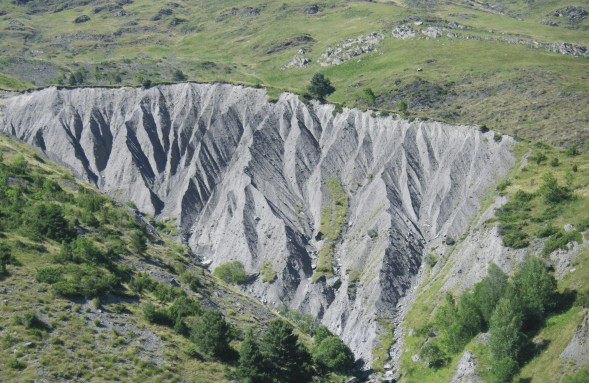
\includegraphics[width=5cm]{Images/Diapos/Erosion/Fluviale/bad_lands.jpg}
    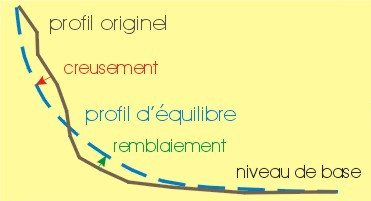
\includegraphics[width=6cm]{Images/Diapos/Erosion/Fluviale/n_base.jpg}
    \caption{Ruissellement et érosion verticale}
  \end{figure}
  \begin{center}
    \begin{figure}
      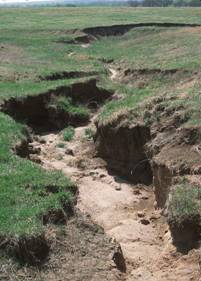
\includegraphics[width=2cm]{Images/Diapos/Erosion/Fluviale/solixfluxion.jpg}
      \caption{Solifluxion}
    \end{figure}
  \end{center}
\end{frame}

\subsection{L'érosion karstique}
\begin{frame}
  \begin{center}
    \begin{figure}[h]
      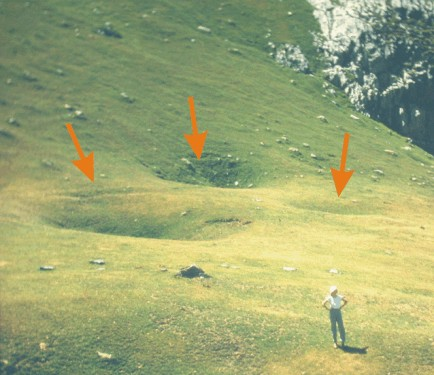
\includegraphics[width=5.35cm]{Images/Diapos/Erosion/Karstique/dolines.jpg}
      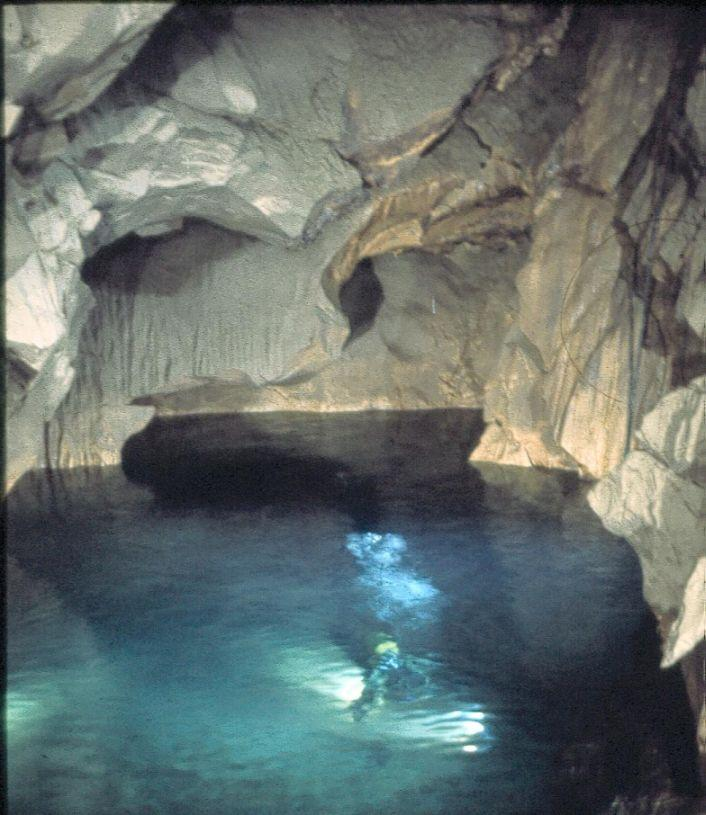
\includegraphics[width=4cm]{Images/Diapos/Erosion/Karstique/erosion-karstique-fig04.jpg}
      \caption{Dolines et grotte souterraine dus à l'érosion karstique.}
    \end{figure}
  \end{center}
\end{frame}

\subsection{L'érosion glaciaire}
\begin{frame}
  \begin{center}
    \begin{figure}
      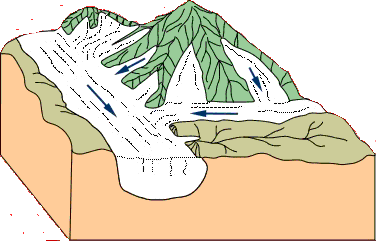
\includegraphics[width=8cm]{Images/Diapos/Erosion/Glaciaire/Erosion_glaciaire_Bourque4B.png}
      \caption{Schéma de l'érosion glaciaire}
    \end{figure}
  \end{center}
\end{frame}

\section{Les simulations}
\subsection{Le système cellulaire}
\begin{frame}
  \begin{center}
    \begin{figure}
      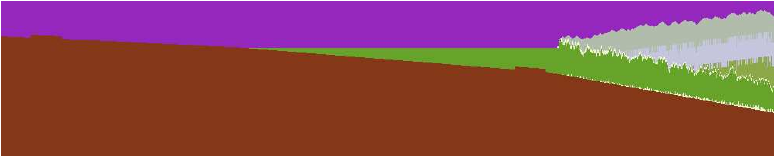
\includegraphics[width=10cm]{Images/3100_cell.png}
      \caption{Simulation par automate cellulaire après 3100 itérations.}
    \end{figure}
    \begin{figure}
      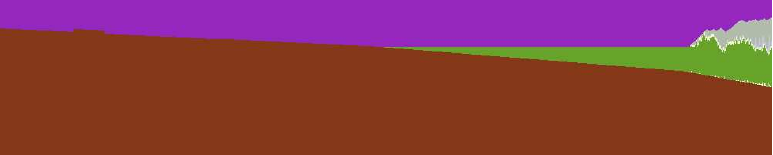
\includegraphics[width=10cm]{Images/7100_cell.png}
      \caption{Simulation par automate cellulaire après 7100 itérations.}
    \end{figure}
  \end{center}
\end{frame}

\subsection{Les cellules}
\begin{frame}
  Cellule : plus petit élément incompressible, sphère de diamètre 1. \smallbreak
  Propriétés mutables :
  \begin{itemize}
   \item vélocité~;
   \item position~;
   \item cellules adjacentes.
  \end{itemize}
  Propriétés immuables :
  \begin{itemize}
   \item plaque tectonique.
  \end{itemize}
  \begin{figure}
    \begin{center}
      
\includegraphics[width=2cm]{Images/cellule.png}
    \end{center}
    \caption{Représentation de 2 cellules.}
  \end{figure}
\end{frame}

\subsection{La disposition des cellules}
\begin{frame}
  Disposition en nid-d'abeille au lancement de la simulation, équidistance de 1 entre cellules.
  \begin{center}
    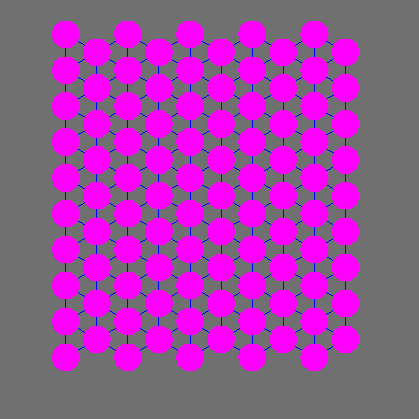
\includegraphics[width=4cm]{Images/hexagone.png}
  \end{center}
  Pour $n_{max}$ cellules en $x$ et $y$ : \\
  \begin{center}
    $x_{max} = n_{max}$ \\
    $x_{min} = n_{max} - 1$ \\
    $y = n \times \sin{\frac{\pi}{3}}$
  \end{center}
\end{frame}

\subsection{Les interaction entre cellules}
\begin{frame}
\begin{figure}
\begin{center}
\begin{tikzpicture}[line cap=round,line join=round,>=triangle 45,x=1.0cm,y=1.0cm,scale=0.5,every node/.style={scale=0.8}]
\clip(-2.25,-2.25) rectangle (21.25,6);
\draw(0,2.83) circle (2cm);
\draw(2.83,0) circle (2cm);
\draw(7,2.83) circle (2cm);
\draw(9.83,0) circle (2cm);
\draw(15,2) circle (2cm);
\draw(19,2) circle (2cm);
\draw [->] (0,2.83) -- (0,1);
\draw [->] (2.83,0) -- (4.09,-1.26);
\draw [->] (9.83,0) -- (8.75,1.09);
\draw [->] (7,2.83) -- (7,4.83);
\draw [->] (15,2) -- (15,4);
\draw [->] (19,2) -- (19,3);
\begin{scriptsize}
\fill [color=qqqqff] (0,2.83) circle (1.5pt);
\draw[color=qqqqff] (0.42,3.21) node {$C_1$};
\fill [color=qqqqff] (2.83,0) circle (1.5pt);
\draw[color=qqqqff] (3.27,0.36) node {$C_2$};
\fill [color=qqqqff] (7,2.83) circle (1.5pt);
\draw[color=qqqqff] (7.42,3.21) node {$C_1$};
\fill [color=qqqqff] (9.83,0) circle (1.5pt);
\draw[color=qqqqff] (10.24,0.36) node {$C_2$};
\fill [color=qqqqff] (15,2) circle (1.5pt);
\draw[color=qqqqff] (15.42,2.36) node {$C_1$};
\fill [color=qqqqff] (19,2) circle (1.5pt);
\draw[color=qqqqff] (19.44,2.36) node {$C_2$};
\draw[color=black] (0.19,2.13) node {$u$};
\draw[color=black] (3.61,-0.35) node {$?$};
\draw[color=black] (9.66,0.6) node {$?$};
\draw[color=black] (7.14,4.04) node {$z$};
\draw[color=black] (14.91,3.21) node {$i$};
\draw[color=black] (18.63,2.73) node {$?$};
\end{scriptsize}
\end{tikzpicture}
\end{center}
\caption{Trois interactions différentes entre cellules : 1) Compression ; 2) Traction ; 3) Friction.}
\end{figure}
\end{frame}

\subsection{Le centre instantané de rotation}
\begin{frame}
  \begin{multicols}{2}
    \begin{center}
      \begin{tikzpicture}[line cap=round,line join=round,>=triangle 45,x=0.4cm,y=0.4cm,scale=0.65,every node/.style={scale=0.65}]
      \clip(-5,-5) rectangle (17,12);
      \draw [shift={(16.25,7)},color=qqwuqq,fill=qqwuqq,fill opacity=0.1] (0,0) -- (-150.26:4.15) arc (-150.26:-139.13:4.15) -- cycle;
      \draw [shift={(16.25,7)},color=qqwuqq,fill=qqwuqq,fill opacity=0.1] (0,0) -- (180:4.15) arc (180:191.31:4.15) -- cycle;
      \draw[color=qqwuqq,fill=qqwuqq,fill opacity=0.1] (0.88,7) -- (0.88,7.88) -- (0,7.88) -- (0,7) -- cycle; 
      \draw[color=qqwuqq,fill=qqwuqq,fill opacity=0.1] (4.76,0.44) -- (4.33,1.2) -- (3.56,0.76) -- (4,0) -- cycle; 
      \draw (0,-2) -- (0,12);
      \draw [domain=-4:16] plot(\x,{(-0-0*\x)/4});
      \draw [->] (0,7) -- (0,3.75);
      \draw(0,7) circle (2cm);
      \draw(4,0) circle (2cm);
      \draw [domain=-4:16] plot(\x,{(--28-7*\x)/4});
      \draw [->] (4,0) -- (5.38,-2.41);
      \draw (0,7)-- (16.25,7);
      \draw (16.25,7)-- (4,0);
      \draw (5.38,-2.41)-- (16.25,7);
      \draw (0,3.75)-- (16.25,7);
      \draw [->] (0,7) -- (4,0);
      \begin{scriptsize}
      \draw[color=black] (0.27,5.65) node {$u$};
      \draw[color=black] (4.92,-0.84) node {$v$};
      \fill [color=uququq] (16.25,7) circle (1.5pt);
      \draw[color=uququq] (16.59,7.53) node {$C$};
      \draw[color=black] (8.28,6.67) node {$d$};
      \draw[color=black] (9.86,4.32) node {$f$};
      \draw[color=qqwuqq] (14.76,5.69) node {$\beta$};
      \draw[color=qqwuqq] (14.47,6.86) node {$\alpha$};
      \draw[color=black] (2.26,3.85) node {$w$};
      \end{scriptsize}
      \end{tikzpicture}
    \end{center}    \vfill
    \columnbreak
    $\overrightarrow{u} = $ vélocité verticale \smallbreak
    $\overrightarrow{v} = $ vélocité horizontale \smallbreak
    $\alpha = \beta = $ rotation autour de F \smallbreak
    $||\overrightarrow{u}|| = \alpha \times d$ \smallbreak
    $||\overrightarrow{v}|| = \alpha \times f$ \smallbreak
    $\alpha = \frac{||\overrightarrow{u}||}{d}$ \smallbreak
  \end{multicols}
\end{frame}

\begin{frame}
  \begin{figure}
    \begin{center}
      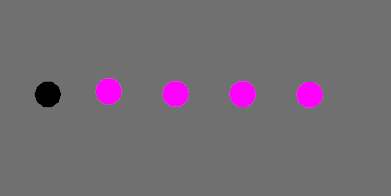
\includegraphics[width=3.5cm]{Images/cir_1.png}
      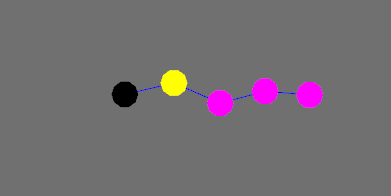
\includegraphics[width=3.5cm]{Images/cir_2.png}
      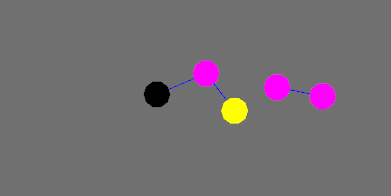
\includegraphics[width=3.5cm]{Images/cir_3.png}
    \end{center}
    \begin{center}
      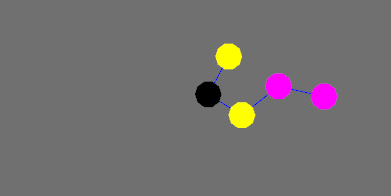
\includegraphics[width=3.5cm]{Images/cir_4.png}
      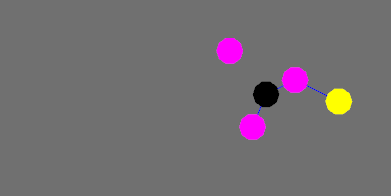
\includegraphics[width=3.5cm]{Images/cir_5.png}
      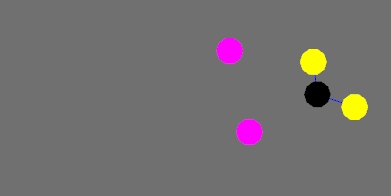
\includegraphics[width=3.5cm]{Images/cir_6.png}
    \end{center}
    \caption{6 échantillons de compressions avec le CIR.}
  \end{figure}
\end{frame}

\subsection{La compression}
\begin{frame}
  \begin{center}
    $\sigma = E \times \varepsilon$
  \end{center}
  $\sigma = $ Contrainte appliquée sur le matériau (en Pa). $E = $ Module de Young pour le matériau étudié (en Pa). $\varepsilon = $ Coefficient de déformation (en $\%$). \smallbreak
  Module de Young :
  \begin{itemize}
    \item Granite : 60 GPa ;
    \item Calcaire : 20 à 70 GPa.
  \end{itemize}
  \smallbreak
  \begin{center}
    Si traction : $d' \leqslant 0 \Rightarrow \sigma = -d'^2$ \medbreak
    Si compression : $d' > 0 \Rightarrow \sigma = d'^2$
  \end{center}
  $d'$ = $1 -$ la distance entre les deux cellules. \\
\end{frame}

\begin{frame}
  \begin{figure}
    \begin{center}
      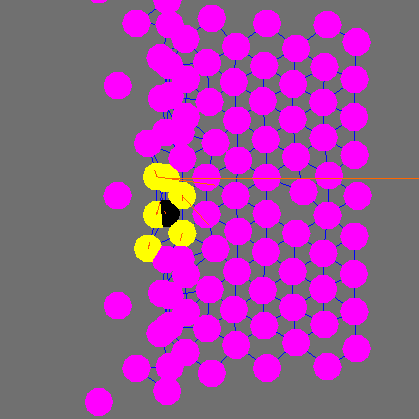
\includegraphics[width=3cm]{Images/normal_1.png}
      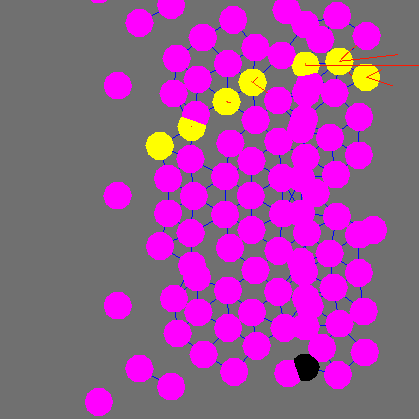
\includegraphics[width=3cm]{Images/normal_2.png}
    \end{center}
    \caption{Simulation sans compression.}
  \end{figure}
  \begin{figure}
    \begin{center}
      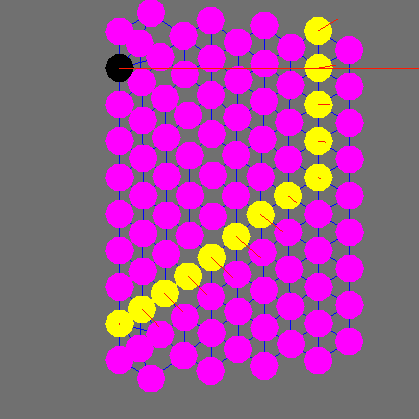
\includegraphics[width=3cm]{Images/compression_1.png}
      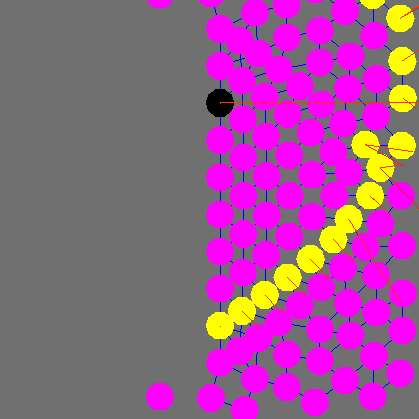
\includegraphics[width=3cm]{Images/compression_2.png}
    \end{center}
    \caption{Simulation avec compression.}
  \end{figure}
\end{frame}

\subsection{La propagation par fronts}
\begin{frame}
  Propagation par front, l’ancien front crée le nouveau. Le premier front ne contient que la cellule en collision.
  Chaque cellule du front interagit avec les cellules qui précèdent le front.
  \begin{figure}
    \begin{center}
      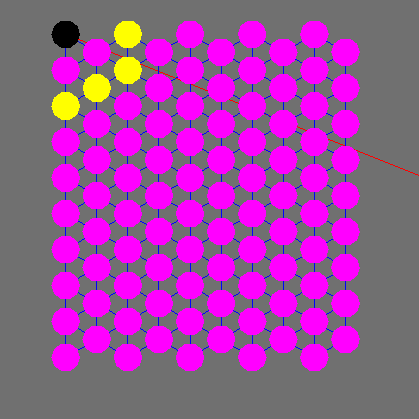
\includegraphics[width=2.5cm]{Images/front_1.png}
      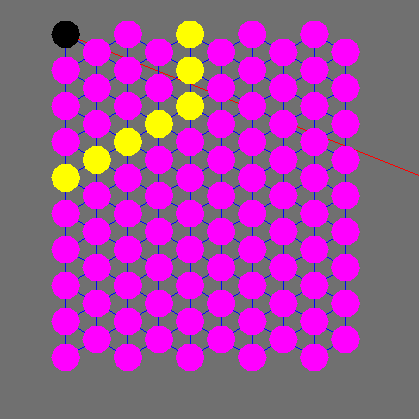
\includegraphics[width=2.5cm]{Images/front_2.png}
      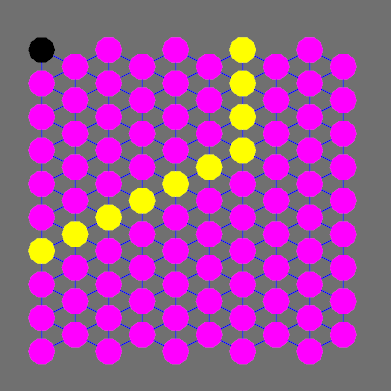
\includegraphics[width=2.5cm]{Images/front_3.png}
    \end{center}
    \begin{center}
      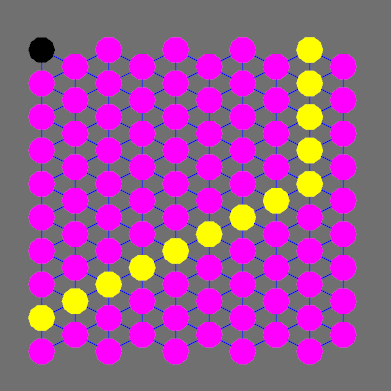
\includegraphics[width=2.5cm]{Images/front_4.png}
      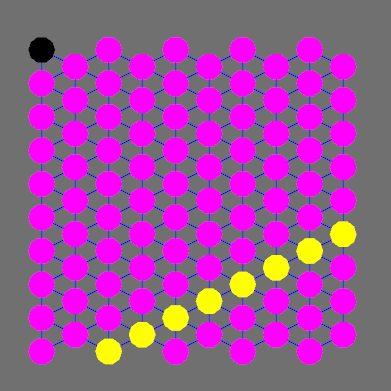
\includegraphics[width=2.5cm]{Images/front_5.png}
      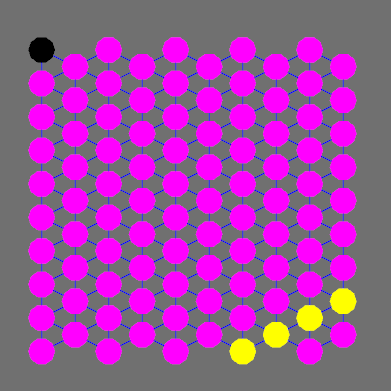
\includegraphics[width=2.5cm]{Images/front_6.png}
    \end{center}

    \caption{Bleu : liens entre cellules, Violet : cellules inactives, Noir : cellule de collision, Jaune : cellules appartenant au front.}
  \end{figure}
\end{frame}

\begin{frame}
  Utilisation d'un calque pour chaque cellule en collision. Fusion des calques avant le déplacement des cellules.
  \begin{figure}
    \begin{center}
      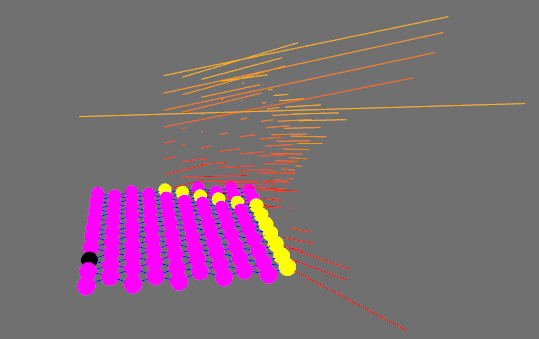
\includegraphics[width=6cm]{Images/calque.png}
    \end{center}
    \caption{Du rouge vers le jaune les différentes vélocités par cellules et par collisions.}
  \end{figure}
\end{frame}

\subsection{La friction}
\begin{frame}
  \begin{center}
    $T_0 = f_0 \times N$
  \end{center}
  Si $T > T_0$ : glissement. Sinon friction. \smallbreak
  Où $T = $ : force tangentielle, $N = $ : contrainte à la normale, $f_0 = $ : coefficient d'adhérence.
  \begin{figure}
    \begin{center}
      \begin{tikzpicture}[line cap=round,line join=round,>=triangle 45,x=0.8cm,y=1.0cm]
	\clip(-4,-1) rectangle (4,2);
	\draw [shift={(0,0)},color=qqwuqq,fill=qqwuqq,fill opacity=0.1] (0,0) -- (53.13:0.63) arc (53.13:126.87:0.63) -- cycle;
	\draw (-1.5,2)-- (0,0);
	\draw (0,0)-- (1.5,2);
	\draw (1.5,2)-- (-1.5,2);
	\draw [domain=-4:4] plot(\x,{(-0-0*\x)/4});
	\draw (0,0)-- (0,1.41);
	\draw (-1.06,1.41)-- (1.06,1.41);
	\begin{scriptsize}
	  \draw[color=qqwuqq] (0.1,0.4) node {$f_0$};
	  \draw[color=black] (0.21,0.79) node {$N$};
	  \draw[color=black] (0.1,1.55) node {$T$};
	\end{scriptsize}
      \end{tikzpicture}
    \end{center}
    \caption{Le cône représentant la force maximale possible avant un glissement.}
  \end{figure}
\end{frame}

\subsection{Les limites matérielles}
\begin{frame}
  
\end{frame}

\section{Les Améliorations possibles}
\begin{frame}
  Améliorations :
  \begin{itemize}
    \item implémenter l'érosion ;
    \item utilisation de la loi de Hooke et du module de Young~;
    \item utilisation d'un modèle avec friction grâce a la loi de Coulomb~;
    \item implémentation de l'inertie des cellules en fonction de leur masse.
  \end{itemize}
\end{frame}

\section{Conclusion}
\begin{frame}
 
\end{frame}


\end{document}
